\subsection{Ausgabeknoten}

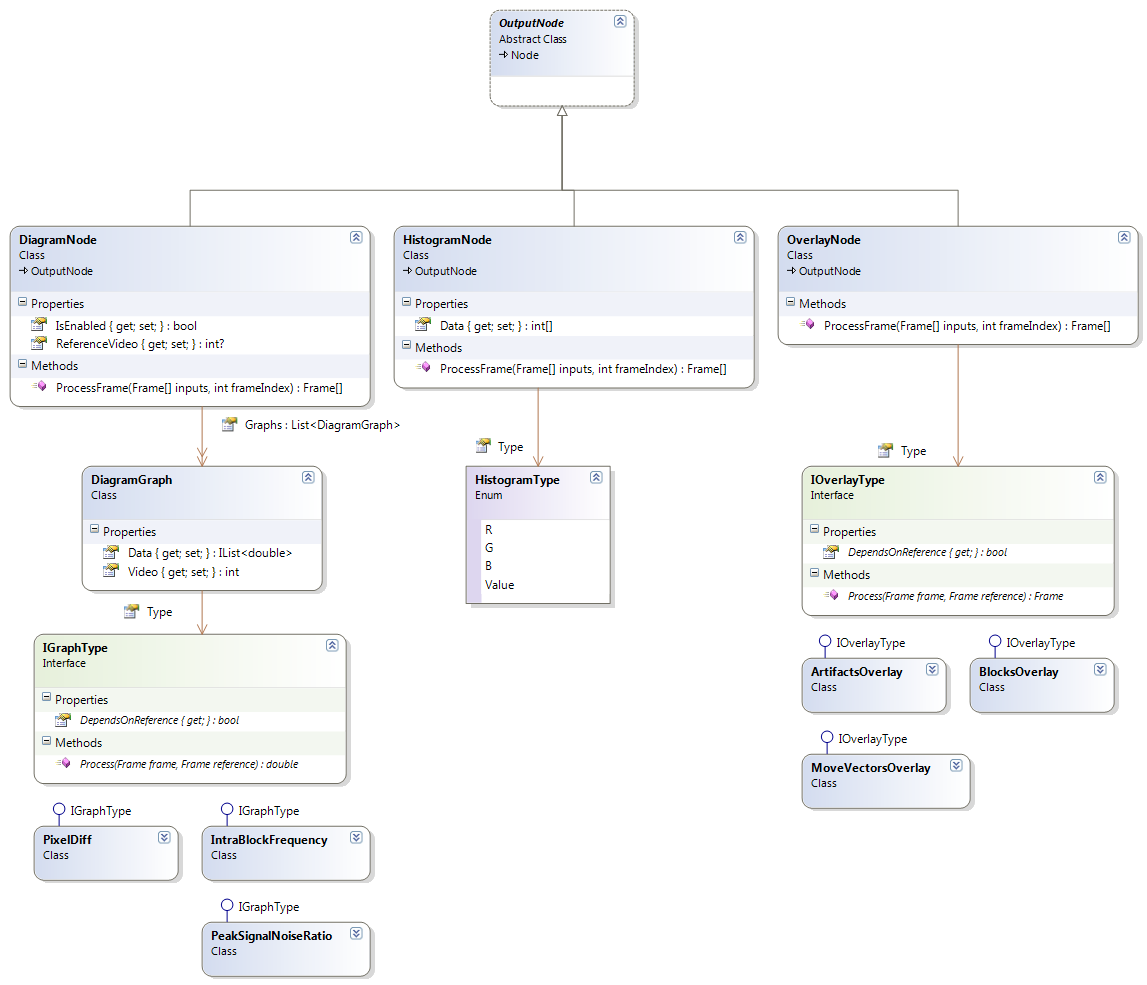
\includegraphics[width=\textwidth]{YuvKA.Pipeline/outputnodes.png}
Die folgenden Klassen stellen Knoten zur Verfügung, die die Ausgabe und Analyse der Videos der Pipeline übernehmen. All diese Klassen erben von der abstrakten Klasse \name{OutputNode}, welche wiederum von der abstrakten Klasse \name{Node} erbt.

\subsubsection{YuvKA.Pipeline.OutputNode}

\begin{verbatim}
public abstract class OutputNode : Node
\end{verbatim}

\paragraph{Beschreibung}~\\
Die abstrakte Klasse \name{OutputNode} modelliert die Ausgabemöglichkeiten der Pipeline und bietet eine gemeinsame Basis für deren konkrete Implementationen.

\subsubsection{YuvKA.Pipeline.DiagramNode}

\subsubsection{YuvKA.Pipeline.HistogramNode}

\begin{verbatim}
public class HistogramNode : OutputNode
\end{verbatim}
Die Klasse \name{HistogramNode} stellt die Daten zur Verfügung, die von dem \name{HistogramViewModel} verwendet werden, um die Histogrammgrafiken darzustellen. Es werden für jeden der drei Farbkanäle sowie für für den Farbwert V im HSV-Raum jeweils ein Histogramm unterstützt.

\paragraph{Typmember}
\begin{itemize}
\property{Type}
	\begin{verbatim}
		[Browsable(false)]
		public HistogramType Type
	\end{verbatim}
	Ruft den Histogrammtyp ab oder legt ihn fest. Es werden vier Arten von Histogrammen unterstützt: jeweils einen für jeden der drei Farbkanäle, sowie einen für den Farbwert im HSV-Raum.
	
\property{Data}
	\begin{verbatim}
		[Browsable(false)]
		public double[] Data { get; }
	\end{verbatim}
	Ruft ein Array der Größe 256 ab, in dem die Verteilung des Farbkanals oder HSV-Farbwerts im \name{Frame} dargestellt ist. Die Stelle $ i \ (0 \leq i \leq 255) $ im Array speichert die Häufigkeit des Farbwerts $ i $ im \name{Frame} für den gewählten Farb\name{typ} (R, G, B oder V). Der Wert liegt zwischen 0.0 und 1.0, da eine relative Häufigkeit dargestellt wird.

\method{ProcessFrame}
	\begin{verbatim}
		public override Frame[] ProcessFrame(Frame[] inputs, int tick)
	\end{verbatim}
	Die Methode \name{ProcessFrame} berechnet für den angegebenen Histogramm\name{typ} die Häufigkeit der Farbwerte von 0 bis 255 und speichert diese an der entsprechenden Stelle im Array \name{Data}, wie im folgenden Algorithmus zu sehen ist:
	\floatname{algorithm}{Algorithmus}
	\begin{algorithm}[H]
		\caption{Berechnung der relativen Häufigkeit eines Farbtyps}
		\begin{algorithmic}[1]
			\REQUIRE $ PIXELS, $ \COMMENT { Die Menge aller Pixel im Frame.}
			\STATE \COMMENT{ Sei $ f_{t}(p) $ der Wert der Farbe $ t $ im Pixel $ p \ (t \in \{ R, G, B, V \})$, $ t $ festgesetzt in \name{Type}. \\ $ D_i $ entspricht dem \textbf{Data} Array.}
			\FORALL{$ p \in PIXELS $}
				\STATE $ i \gets f_{t}(p) $
				\STATE $ D_i \gets D_i + 1 $
			\ENDFOR
			\FOR{$ i \gets 0 \text{\textbf{ to }} 255 $}
				\STATE $ D_i \gets \frac{D_i}{|PIXELS|} $
			\ENDFOR
			\ENSURE $ D_i, $ \COMMENT { Das Ausgabearray, in dem die Verteilung gespeichert ist.}
		\end{algorithmic}
	\end{algorithm}

\end{itemize}

\subsubsection{YuvKA.Pipeline.OverlayNode}

\begin{verbatim}
[DataContract]
public class OverlayNode : OutputNode
\end{verbatim}

\paragraph{Beschreibung}~\\
Die Klasse \name{OverlayNode} modelliert das überlagern von Videos mit graphischen Darstellungen von Analysedaten.

\paragraph{Typmember}
\begin{itemize}

\property{Type}
	\begin{verbatim}
	[DataMember]
	public IOverlayType Type { get; set; }
	\end{verbatim}
	Ruft die Art der Überlagerung ab, oder legt sie fest. Standardmäßig werden die Markierung von Artefakten im Vergleich mit einem Referenzvideo, das Anzeigen von Bewegungsvektoren sowie eine Anzeige der Makroblockentscheidungen des Encoders unterstützt.

\method{ProcessFrame}
	\begin{verbatim}
	public override Frame[] ProcessFrame(Frame[] inputs, int tick)
	\end{verbatim}
	Überlagert den übergebenen \name{Frame} mit den durch \name{Type} spezifizierten Daten und gibt den Überlagerten \name{Frame} zurück. Bei den standardmäßig unterstützen Möglichkeiten handelt es sich um:
	\begin{description}
		\item[ArtifactsOverlay]~\\
			Für diese Überlagerung werden zwei Eingabeframes benötigt, da hier die Artefakte eines \name{Frame}s im Vergleich mit einem anderen hervorgehoben werden.
		\item[BlocksOverlay]~\\
			Für diese Überlagerung wird eine Eingabe in Form eines \name{AnnotatedFrame}s benötigt, da aus den Logdateien die Makroblockentscheidungen des Encoders entnommen werden um damit die Darstellung dieser Entscheidungen über dem \name{Frame} zu legen.
		\item[MoveVectorsOverlay]~\\
			Für diese Überlagerung wird eine Eingabe in Form eines \name{AnnotatedFrame}s benötigt, da aus den Logdateien die erkannten Bewegungsvektoren des Encoders entnommen werden um diese in den \name{Frame} einzuzeichnen.
	\end{description}
	
\end{itemize}